% --------------------------------------------------------------
% This is all preamble stuff that you don't have to worry about.
% Head down to where it says "Start here"
% --------------------------------------------------------------
\documentclass[paper=a4, fontsize=11pt]{scrartcl} % A4 paper and 11pt font size 

\usepackage[T1]{fontenc} % Use 8-bit encoding that has 256 glyphs
\usepackage{fourier} % Use the Adobe Utopia font for the document - comment this line to return to the LaTeX default
\usepackage[english]{babel} % English language/hyphenation
\usepackage{mathtools} 
\usepackage{sectsty}
\usepackage{hyperref}
\usepackage[margin=1in]{geometry} 
\usepackage{amsmath,amsthm,amssymb}
 \usepackage{enumerate}
\usepackage{graphicx}
\hypersetup{
    colorlinks=true,
    linkcolor=blue,
    filecolor=magenta,      
    urlcolor=blue,
}
\usepackage[framed,numbered,autolinebreaks,useliterate]{mcode}

\theoremstyle{plain}

\setlength\parindent{0pt} 

\newcommand{\N}{\mathcal{N}}
\newcommand{\Z}{\mathbb{Z}}
\newcommand{\R}{\mathbb{R}}
\newcommand{\C}{\mathbb{C}}
\newcommand{\E}{\mathbb{E}}

\newtheorem{theorem}{Theorem}
\newtheorem*{lemma*}{lemma}
\newtheorem{corollary}[theorem]{Corollary}
\newtheorem{proposition}[theorem]{Proposition}

\newenvironment{problem}[2][Problem]{\begin{trivlist}
\item[\hskip \labelsep {\bfseries #1}\hskip \labelsep {\bfseries #2:}]}{\end{trivlist}}


\theoremstyle{remark}
\newtheorem*{solution}{Solution}
\newtheorem{example}{Example}

\DeclareMathOperator{\lcm}{lcm}
\DeclareMathOperator{\Aut}{Aut}
\newcommand{\Jac}[3]{{\left(\dfrac{#1}{#2}\right)}}
\newcommand{\norm}[1]{\left\lVert#1\right\rVert}
\usepackage{fancyvrb}

 
\begin{document}
 
\newcommand{\horrule}[1]{\rule{\linewidth}{#1}} % Create horizontal rule command with 1 argument of height

\title{	
\normalfont \normalsize 
\textsc{Early Graduate Research} \\ [25pt] % Your university, school and/or department name(s)
\horrule{0.5pt} \\[0.4cm] % Thin top horizontal rule
\huge Weekly Report 01  \\ % The assignment title
\horrule{2pt} \\[0.5cm] % Thick bottom horizontal rule
}

\author{Michael Dairyko and Caleb Logemann } % Your name
\date{}

 

\maketitle


%%%%%%%%%%%%%%%%%%%%%%%%%%

This week we studied Chapter 6 from {\em Numerical Methods for Stochastic Compuatations} which discussed the Stochastic Galerkin Method. Specifically we worked on understanding an example of the method using an ODE. We also began to look into the Hamilton-Jacobi Equation and how it is derived.

\begin{section}{Galerkin Method}
The Galerkin method is used for solving stochastic systems. Overall, it is an approximation method that utilizes the inner product of orthogonal polynomials and basis functions. The following example is from section 6.2 of {\em Numerical Methods for Stochastic Compuatations.}

\begin{example}
Illustrate the main steps of the gPC Galerkin method for 
$$\frac{du}{dt} (t,Z) = - \alpha(Z)u, \quad u(t = 0, Z) = \beta.$$ where the initial condition is assumed to be deterministic. We also assume that the random rate constant follows a normal distribution, $\alpha \sim \N(\mu, \sigma^2).$ The corresponding gPC basis will be the Hermite polynomials. Since $\alpha$ is the only random input, we need only univariate gPC Hermite expansion $\{H_k(Z)\}_{k=0}^N,$ $N>0,$ where $Z\sim \N(0,1)$ is the standard normal random variable with zero mean and unit variance. The constant $\alpha$ can be expressed as $\alpha  = \mu + \sigma Z.$ Observe that this is like a change of basis, highlighted by:

$$ 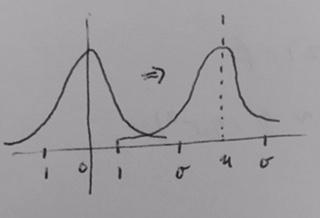
\includegraphics[height=4cm]{ex1} $$

Also notice that $H_0(Z) = 1$ and $H_1(Z) = Z$ Therefore it follows that 

\begin{align*}
\alpha_N(Z) & = \mu + \sigma Z \\
		  & = \mu H_0(Z) + \sigma H_1(Z) \\
		  & = \sum_{i=0}^N a_i H_i(Z),
\end{align*}
where $a_0 = \mu,$ $a_1 = \sigma,$ and $a_i =0$ for all $i\ge 2.$ In this particular case, there is no error term for $N\ge 1,$ meaning that $\alpha_N$ is exact. Now let $$v_N(t,Z) = \sum_{i=0}^N \hat{v}_i (t) \Phi_i(Z)$$ be the $N$th-degree gPC approximation we seek. By initial conditions, $\gamma_0 = 1,$ so

$$\hat{v}_0 = \dfrac{\E[u_0 H_0]}{\gamma_0} = \E[\beta] = \beta.$$

Notice that $\gamma_1 = \E[Z^2] = var(Z) + \E[Z]^2 = \sigma^2 + 1,$ so
$$\hat{v}_1 = \dfrac{\E[u_0 H_1]}{\gamma_1} = \dfrac{\E[\beta Z]}{\sigma^2 + 1} $$

STUCK HERE :(

The gPC Galerkin procedure results in $$\E\left[ \frac{d v_n}{dt} H_k \right] = \E\left[ -\alpha_N v_N H_k\right], \quad \forall \; k = 0,\ldots, N.$$

\end{example}


\end{section}


\end{document}